\documentclass[1p]{elsarticle_modified}
%\bibliographystyle{elsarticle-num}

%\usepackage[colorlinks]{hyperref}
%\usepackage{abbrmath_seonhwa} %\Abb, \Ascr, \Acal ,\Abf, \Afrak
\usepackage{amsfonts}
\usepackage{amssymb}
\usepackage{amsmath}
\usepackage{amsthm}
\usepackage{scalefnt}
\usepackage{amsbsy}
\usepackage{kotex}
\usepackage{caption}
\usepackage{subfig}
\usepackage{color}
\usepackage{graphicx}
\usepackage{xcolor} %% white, black, red, green, blue, cyan, magenta, yellow
\usepackage{float}
\usepackage{setspace}
\usepackage{hyperref}

\usepackage{tikz}
\usetikzlibrary{arrows}

\usepackage{multirow}
\usepackage{array} % fixed length table
\usepackage{hhline}

%%%%%%%%%%%%%%%%%%%%%
\makeatletter
\renewcommand*\env@matrix[1][\arraystretch]{%
	\edef\arraystretch{#1}%
	\hskip -\arraycolsep
	\let\@ifnextchar\new@ifnextchar
	\array{*\c@MaxMatrixCols c}}
\makeatother %https://tex.stackexchange.com/questions/14071/how-can-i-increase-the-line-spacing-in-a-matrix
%%%%%%%%%%%%%%%

\usepackage[normalem]{ulem}

\newcommand{\msout}[1]{\ifmmode\text{\sout{\ensuremath{#1}}}\else\sout{#1}\fi}
%SOURCE: \msout is \stkout macro in https://tex.stackexchange.com/questions/20609/strikeout-in-math-mode

\newcommand{\cancel}[1]{
	\ifmmode
	{\color{red}\msout{#1}}
	\else
	{\color{red}\sout{#1}}
	\fi
}

\newcommand{\add}[1]{
	{\color{blue}\uwave{#1}}
}

\newcommand{\replace}[2]{
	\ifmmode
	{\color{red}\msout{#1}}{\color{blue}\uwave{#2}}
	\else
	{\color{red}\sout{#1}}{\color{blue}\uwave{#2}}
	\fi
}

\newcommand{\Sol}{\mathcal{S}} %segment
\newcommand{\D}{D} %diagram
\newcommand{\A}{\mathcal{A}} %arc


%%%%%%%%%%%%%%%%%%%%%%%%%%%%%5 test

\def\sl{\operatorname{\textup{SL}}(2,\Cbb)}
\def\psl{\operatorname{\textup{PSL}}(2,\Cbb)}
\def\quan{\mkern 1mu \triangleright \mkern 1mu}

\theoremstyle{definition}
\newtheorem{thm}{Theorem}[section]
\newtheorem{prop}[thm]{Proposition}
\newtheorem{lem}[thm]{Lemma}
\newtheorem{ques}[thm]{Question}
\newtheorem{cor}[thm]{Corollary}
\newtheorem{defn}[thm]{Definition}
\newtheorem{exam}[thm]{Example}
\newtheorem{rmk}[thm]{Remark}
\newtheorem{alg}[thm]{Algorithm}

\newcommand{\I}{\sqrt{-1}}
\begin{document}

%\begin{frontmatter}
%
%\title{Boundary parabolic representations of knots up to 8 crossings}
%
%%% Group authors per affiliation:
%\author{Yunhi Cho} 
%\address{Department of Mathematics, University of Seoul, Seoul, Korea}
%\ead{yhcho@uos.ac.kr}
%
%
%\author{Seonhwa Kim} %\fnref{s_kim}}
%\address{Center for Geometry and Physics, Institute for Basic Science, Pohang, 37673, Korea}
%\ead{ryeona17@ibs.re.kr}
%
%\author{Hyuk Kim}
%\address{Department of Mathematical Sciences, Seoul National University, Seoul 08826, Korea}
%\ead{hyukkim@snu.ac.kr}
%
%\author{Seokbeom Yoon}
%\address{Department of Mathematical Sciences, Seoul National University, Seoul, 08826,  Korea}
%\ead{sbyoon15@snu.ac.kr}
%
%\begin{abstract}
%We find all boundary parabolic representation of knots up to 8 crossings.
%
%\end{abstract}
%\begin{keyword}
%    \MSC[2010] 57M25 
%\end{keyword}
%
%\end{frontmatter}

%\linenumbers
%\tableofcontents
%
\newcommand\colored[1]{\textcolor{white}{\rule[-0.35ex]{0.8em}{1.4ex}}\kern-0.8em\color{red} #1}%
%\newcommand\colored[1]{\textcolor{white}{ #1}\kern-2.17ex	\textcolor{white}{ #1}\kern-1.81ex	\textcolor{white}{ #1}\kern-2.15ex\color{red}#1	}

{\Large $\underline{12a_{0131}~(K12a_{0131})}$}

\setlength{\tabcolsep}{10pt}
\renewcommand{\arraystretch}{1.6}
\vspace{1cm}\begin{tabular}{m{100pt}>{\centering\arraybackslash}m{274pt}}
\multirow{5}{120pt}{
	\centering
	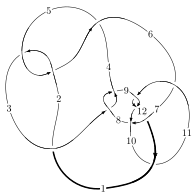
\includegraphics[width=112pt]{../../../GIT/diagram.site/Diagrams/png/932_12a_0131.png}\\
\ \ \ A knot diagram\footnotemark}&
\allowdisplaybreaks
\textbf{Linearized knot diagam} \\
\cline{2-2}
 &
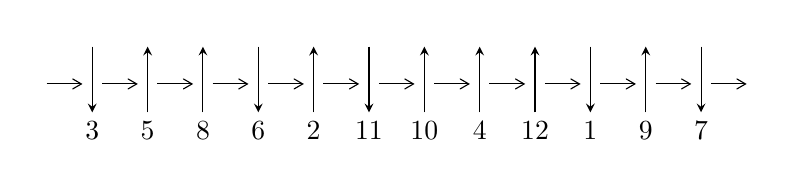
\begin{tikzpicture}[x=20pt, y=17pt]
	% nodes
	\node (C0) at (0, 0) {};
	\node (C1) at (1, 0) {};
	\node (C1U) at (1, +1) {};
	\node (C1D) at (1, -1) {3};

	\node (C2) at (2, 0) {};
	\node (C2U) at (2, +1) {};
	\node (C2D) at (2, -1) {5};

	\node (C3) at (3, 0) {};
	\node (C3U) at (3, +1) {};
	\node (C3D) at (3, -1) {8};

	\node (C4) at (4, 0) {};
	\node (C4U) at (4, +1) {};
	\node (C4D) at (4, -1) {6};

	\node (C5) at (5, 0) {};
	\node (C5U) at (5, +1) {};
	\node (C5D) at (5, -1) {2};

	\node (C6) at (6, 0) {};
	\node (C6U) at (6, +1) {};
	\node (C6D) at (6, -1) {11};

	\node (C7) at (7, 0) {};
	\node (C7U) at (7, +1) {};
	\node (C7D) at (7, -1) {10};

	\node (C8) at (8, 0) {};
	\node (C8U) at (8, +1) {};
	\node (C8D) at (8, -1) {4};

	\node (C9) at (9, 0) {};
	\node (C9U) at (9, +1) {};
	\node (C9D) at (9, -1) {12};

	\node (C10) at (10, 0) {};
	\node (C10U) at (10, +1) {};
	\node (C10D) at (10, -1) {1};

	\node (C11) at (11, 0) {};
	\node (C11U) at (11, +1) {};
	\node (C11D) at (11, -1) {9};

	\node (C12) at (12, 0) {};
	\node (C12U) at (12, +1) {};
	\node (C12D) at (12, -1) {7};
	\node (C13) at (13, 0) {};

	% arrows
	\draw[->,>={angle 60}]
	(C0) edge (C1) (C1) edge (C2) (C2) edge (C3) (C3) edge (C4) (C4) edge (C5) (C5) edge (C6) (C6) edge (C7) (C7) edge (C8) (C8) edge (C9) (C9) edge (C10) (C10) edge (C11) (C11) edge (C12) (C12) edge (C13) ;	\draw[->,>=stealth]
	(C1U) edge (C1D) (C2D) edge (C2U) (C3D) edge (C3U) (C4U) edge (C4D) (C5D) edge (C5U) (C6U) edge (C6D) (C7D) edge (C7U) (C8D) edge (C8U) (C9D) edge (C9U) (C10U) edge (C10D) (C11D) edge (C11U) (C12U) edge (C12D) ;
	\end{tikzpicture} \\
\hhline{~~} \\& 
\textbf{Solving Sequence} \\ \cline{2-2} 
 &
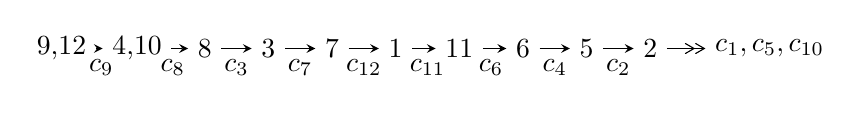
\begin{tikzpicture}[x=23pt, y=7pt]
	% node
	\node (A0) at (-1/8, 0) {9,12};
	\node (A1) at (17/16, 0) {4,10};
	\node (A2) at (17/8, 0) {8};
	\node (A3) at (25/8, 0) {3};
	\node (A4) at (33/8, 0) {7};
	\node (A5) at (41/8, 0) {1};
	\node (A6) at (49/8, 0) {11};
	\node (A7) at (57/8, 0) {6};
	\node (A8) at (65/8, 0) {5};
	\node (A9) at (73/8, 0) {2};
	\node (C1) at (1/2, -1) {$c_{9}$};
	\node (C2) at (13/8, -1) {$c_{8}$};
	\node (C3) at (21/8, -1) {$c_{3}$};
	\node (C4) at (29/8, -1) {$c_{7}$};
	\node (C5) at (37/8, -1) {$c_{12}$};
	\node (C6) at (45/8, -1) {$c_{11}$};
	\node (C7) at (53/8, -1) {$c_{6}$};
	\node (C8) at (61/8, -1) {$c_{4}$};
	\node (C9) at (69/8, -1) {$c_{2}$};
	\node (A10) at (11, 0) {$c_{1},c_{5},c_{10}$};

	% edge
	\draw[->,>=stealth]	
	(A0) edge (A1) (A1) edge (A2) (A2) edge (A3) (A3) edge (A4) (A4) edge (A5) (A5) edge (A6) (A6) edge (A7) (A7) edge (A8) (A8) edge (A9) ;
	\draw[->>,>={angle 60}]	
	(A9) edge (A10);
\end{tikzpicture} \\ 

\end{tabular} \\

\footnotetext{
The image of knot diagram is generated by the software ``\textbf{Draw programme}" developed by Andrew Bartholomew(\url{http://www.layer8.co.uk/maths/draw/index.htm\#Running-draw}), where we modified some parts for our purpose(\url{https://github.com/CATsTAILs/LinksPainter}).
}\phantom \\ \newline 
\centering \textbf{Ideals for irreducible components\footnotemark of $X_{\text{par}}$} 
 
\begin{align*}
I^u_{1}&=\langle 
2.64768\times10^{518} u^{124}-8.42800\times10^{518} u^{123}+\cdots+4.89215\times10^{516} b+1.49453\times10^{519},\\
\phantom{I^u_{1}}&\phantom{= \langle  }3.73739\times10^{519} u^{124}-1.18654\times10^{520} u^{123}+\cdots+9.78430\times10^{516} a+2.09349\times10^{520},\\
\phantom{I^u_{1}}&\phantom{= \langle  }u^{125}-3 u^{124}+\cdots+17 u+1\rangle \\
I^u_{2}&=\langle 
b,\;- u^5 a+2 u^4 a+u^5-3 u^4-2 u^2 a+3 u^3+a^2+a u-2 u+1,\;u^6- u^5- u^4+2 u^3- u+1\rangle \\
\\
\end{align*}
\raggedright * 2 irreducible components of $\dim_{\mathbb{C}}=0$, with total 137 representations.\\
\footnotetext{All coefficients of polynomials are rational numbers. But the coefficients are sometimes approximated in decimal forms when there is not enough margin.}
\newpage
\renewcommand{\arraystretch}{1}
\centering \section*{I. $I^u_{1}= \langle 2.65\times10^{518} u^{124}-8.43\times10^{518} u^{123}+\cdots+4.89\times10^{516} b+1.49\times10^{519},\;3.74\times10^{519} u^{124}-1.19\times10^{520} u^{123}+\cdots+9.78\times10^{516} a+2.09\times10^{520},\;u^{125}-3 u^{124}+\cdots+17 u+1 \rangle$}
\flushleft \textbf{(i) Arc colorings}\\
\begin{tabular}{m{7pt} m{180pt} m{7pt} m{180pt} }
\flushright $a_{9}=$&$\begin{pmatrix}1\\0\end{pmatrix}$ \\
\flushright $a_{12}=$&$\begin{pmatrix}0\\u\end{pmatrix}$ \\
\flushright $a_{4}=$&$\begin{pmatrix}-381.979 u^{124}+1212.70 u^{123}+\cdots-24299.3 u-2139.65\\-54.1209 u^{124}+172.276 u^{123}+\cdots-3476.17 u-305.495\end{pmatrix}$ \\
\flushright $a_{10}=$&$\begin{pmatrix}1\\- u^2\end{pmatrix}$ \\
\flushright $a_{8}=$&$\begin{pmatrix}182.743 u^{124}-578.359 u^{123}+\cdots+11566.7 u+1015.20\\12.4867 u^{124}-41.0452 u^{123}+\cdots+888.570 u+77.2473\end{pmatrix}$ \\
\flushright $a_{3}=$&$\begin{pmatrix}-525.800 u^{124}+1672.25 u^{123}+\cdots-33602.3 u-2955.69\\-87.0132 u^{124}+275.060 u^{123}+\cdots-5477.59 u-481.773\end{pmatrix}$ \\
\flushright $a_{7}=$&$\begin{pmatrix}162.525 u^{124}-515.547 u^{123}+\cdots+10348.7 u+907.820\\14.2770 u^{124}-45.0112 u^{123}+\cdots+905.020 u+79.4042\end{pmatrix}$ \\
\flushright $a_{1}=$&$\begin{pmatrix}-136.294 u^{124}+433.527 u^{123}+\cdots-8784.44 u-770.986\\-24.6461 u^{124}+77.8439 u^{123}+\cdots-1546.01 u-136.294\end{pmatrix}$ \\
\flushright $a_{11}=$&$\begin{pmatrix}- u\\u\end{pmatrix}$ \\
\flushright $a_{6}=$&$\begin{pmatrix}169.080 u^{124}-534.889 u^{123}+\cdots+10684.5 u+937.972\\7.72249 u^{124}-25.6696 u^{123}+\cdots+569.242 u+49.2525\end{pmatrix}$ \\
\flushright $a_{5}=$&$\begin{pmatrix}-591.960 u^{124}+1881.43 u^{123}+\cdots-37752.9 u-3321.58\\-94.7243 u^{124}+300.362 u^{123}+\cdots-6018.61 u-528.924\end{pmatrix}$ \\
\flushright $a_{2}=$&$\begin{pmatrix}99.7178 u^{124}-314.202 u^{123}+\cdots+6266.98 u+544.092\\-18.8512 u^{124}+58.0831 u^{123}+\cdots-1084.59 u-96.9655\end{pmatrix}$\\&\end{tabular}
\flushleft \textbf{(ii) Obstruction class $= -1$}\\~\\
\flushleft \textbf{(iii) Cusp Shapes $= -323.549 u^{124}+1024.38 u^{123}+\cdots-20264.6 u-1780.82$}\\~\\
\newpage\renewcommand{\arraystretch}{1}
\flushleft \textbf{(iv) u-Polynomials at the component}\newline \\
\begin{tabular}{m{50pt}|m{274pt}}
Crossings & \hspace{64pt}u-Polynomials at each crossing \\
\hline $$\begin{aligned}c_{1},c_{4}\end{aligned}$$&$\begin{aligned}
&u^{125}+41 u^{124}+\cdots-145 u-1
\end{aligned}$\\
\hline $$\begin{aligned}c_{2},c_{5}\end{aligned}$$&$\begin{aligned}
&u^{125}+7 u^{124}+\cdots-9 u-1
\end{aligned}$\\
\hline $$\begin{aligned}c_{3},c_{8}\end{aligned}$$&$\begin{aligned}
&u^{125}- u^{124}+\cdots+20480 u-4096
\end{aligned}$\\
\hline $$\begin{aligned}c_{6}\end{aligned}$$&$\begin{aligned}
&u^{125}+3 u^{124}+\cdots-6561489 u+604147
\end{aligned}$\\
\hline $$\begin{aligned}c_{7}\end{aligned}$$&$\begin{aligned}
&u^{125}+9 u^{124}+\cdots+391375 u+25489
\end{aligned}$\\
\hline $$\begin{aligned}c_{9},c_{11}\end{aligned}$$&$\begin{aligned}
&u^{125}+3 u^{124}+\cdots+17 u-1
\end{aligned}$\\
\hline $$\begin{aligned}c_{10}\end{aligned}$$&$\begin{aligned}
&u^{125}-21 u^{124}+\cdots-3 u+1
\end{aligned}$\\
\hline $$\begin{aligned}c_{12}\end{aligned}$$&$\begin{aligned}
&u^{125}-9 u^{124}+\cdots-3 u+1
\end{aligned}$\\
\hline
\end{tabular}\\~\\
\newpage\renewcommand{\arraystretch}{1}
\flushleft \textbf{(v) Riley Polynomials at the component}\newline \\
\begin{tabular}{m{50pt}|m{274pt}}
Crossings & \hspace{64pt}Riley Polynomials at each crossing \\
\hline $$\begin{aligned}c_{1},c_{4}\end{aligned}$$&$\begin{aligned}
&y^{125}+93 y^{124}+\cdots+5099 y-1
\end{aligned}$\\
\hline $$\begin{aligned}c_{2},c_{5}\end{aligned}$$&$\begin{aligned}
&y^{125}+41 y^{124}+\cdots-145 y-1
\end{aligned}$\\
\hline $$\begin{aligned}c_{3},c_{8}\end{aligned}$$&$\begin{aligned}
&y^{125}-65 y^{124}+\cdots+301989888 y-16777216
\end{aligned}$\\
\hline $$\begin{aligned}c_{6}\end{aligned}$$&$\begin{aligned}
&y^{125}-91 y^{124}+\cdots-24775319389441 y-364993597609
\end{aligned}$\\
\hline $$\begin{aligned}c_{7}\end{aligned}$$&$\begin{aligned}
&y^{125}-127 y^{124}+\cdots+36942460527 y-649689121
\end{aligned}$\\
\hline $$\begin{aligned}c_{9},c_{11}\end{aligned}$$&$\begin{aligned}
&y^{125}-83 y^{124}+\cdots-17 y-1
\end{aligned}$\\
\hline $$\begin{aligned}c_{10}\end{aligned}$$&$\begin{aligned}
&y^{125}-3 y^{124}+\cdots-17 y-1
\end{aligned}$\\
\hline $$\begin{aligned}c_{12}\end{aligned}$$&$\begin{aligned}
&y^{125}+21 y^{124}+\cdots-9 y-1
\end{aligned}$\\
\hline
\end{tabular}\\~\\
\newpage\flushleft \textbf{(vi) Complex Volumes and Cusp Shapes}
$$\begin{array}{c|c|c}  
\text{Solutions to }I^u_{1}& \I (\text{vol} + \sqrt{-1}CS) & \text{Cusp shape}\\
 \hline 
\begin{aligned}
u &= -1.003630 + 0.091762 I \\
a &= -3.97740 - 2.38530 I \\
b &= \phantom{-}0.818217 - 0.461607 I\end{aligned}
 & -0.01102 - 2.45400 I & \phantom{-0.000000 } 0 \\ \hline\begin{aligned}
u &= -1.003630 - 0.091762 I \\
a &= -3.97740 + 2.38530 I \\
b &= \phantom{-}0.818217 + 0.461607 I\end{aligned}
 & -0.01102 + 2.45400 I & \phantom{-0.000000 } 0 \\ \hline\begin{aligned}
u &= -0.982156 + 0.100911 I \\
a &= -2.15785 + 4.64167 I \\
b &= \phantom{-}0.310656 + 0.355934 I\end{aligned}
 & \phantom{-}1.72895 - 2.62928 I & \phantom{-0.000000 } 0 \\ \hline\begin{aligned}
u &= -0.982156 - 0.100911 I \\
a &= -2.15785 - 4.64167 I \\
b &= \phantom{-}0.310656 - 0.355934 I\end{aligned}
 & \phantom{-}1.72895 + 2.62928 I & \phantom{-0.000000 } 0 \\ \hline\begin{aligned}
u &= -0.112173 + 0.977335 I \\
a &= -0.393390 + 1.060410 I \\
b &= \phantom{-}0.267605 + 0.980914 I\end{aligned}
 & \phantom{-}0.76237 - 1.42438 I & \phantom{-0.000000 } 0 \\ \hline\begin{aligned}
u &= -0.112173 - 0.977335 I \\
a &= -0.393390 - 1.060410 I \\
b &= \phantom{-}0.267605 - 0.980914 I\end{aligned}
 & \phantom{-}0.76237 + 1.42438 I & \phantom{-0.000000 } 0 \\ \hline\begin{aligned}
u &= \phantom{-}0.239455 + 0.994751 I \\
a &= \phantom{-}0.314123 - 0.696394 I \\
b &= -0.594765 - 0.685477 I\end{aligned}
 & -4.30119 - 2.18209 I & \phantom{-0.000000 } 0 \\ \hline\begin{aligned}
u &= \phantom{-}0.239455 - 0.994751 I \\
a &= \phantom{-}0.314123 + 0.696394 I \\
b &= -0.594765 + 0.685477 I\end{aligned}
 & -4.30119 + 2.18209 I & \phantom{-0.000000 } 0 \\ \hline\begin{aligned}
u &= \phantom{-}1.013110 + 0.179661 I \\
a &= -2.25528 + 0.34509 I \\
b &= \phantom{-}1.304260 + 0.497331 I\end{aligned}
 & -0.34954 + 4.52947 I & \phantom{-0.000000 } 0 \\ \hline\begin{aligned}
u &= \phantom{-}1.013110 - 0.179661 I \\
a &= -2.25528 - 0.34509 I \\
b &= \phantom{-}1.304260 - 0.497331 I\end{aligned}
 & -0.34954 - 4.52947 I & \phantom{-0.000000 } 0\\
 \hline 
 \end{array}$$\newpage$$\begin{array}{c|c|c}  
\text{Solutions to }I^u_{1}& \I (\text{vol} + \sqrt{-1}CS) & \text{Cusp shape}\\
 \hline 
\begin{aligned}
u &= -1.039630 + 0.023694 I \\
a &= \phantom{-}0.67319 - 3.23584 I \\
b &= \phantom{-}0.130567 + 0.838675 I\end{aligned}
 & \phantom{-}2.45673 - 2.54518 I & \phantom{-0.000000 } 0 \\ \hline\begin{aligned}
u &= -1.039630 - 0.023694 I \\
a &= \phantom{-}0.67319 + 3.23584 I \\
b &= \phantom{-}0.130567 - 0.838675 I\end{aligned}
 & \phantom{-}2.45673 + 2.54518 I & \phantom{-0.000000 } 0 \\ \hline\begin{aligned}
u &= -0.109764 + 1.042850 I \\
a &= -0.728339 - 0.206603 I \\
b &= \phantom{-}1.040380 - 0.309779 I\end{aligned}
 & \phantom{-}1.20280 - 4.30451 I & \phantom{-0.000000 } 0 \\ \hline\begin{aligned}
u &= -0.109764 - 1.042850 I \\
a &= -0.728339 + 0.206603 I \\
b &= \phantom{-}1.040380 + 0.309779 I\end{aligned}
 & \phantom{-}1.20280 + 4.30451 I & \phantom{-0.000000 } 0 \\ \hline\begin{aligned}
u &= -1.05632\phantom{ +0.000000I} \\
a &= \phantom{-}5.26697\phantom{ +0.000000I} \\
b &= -0.911297\phantom{ +0.000000I}\end{aligned}
 & \phantom{-}3.09971\phantom{ +0.000000I} & \phantom{-0.000000 } 0 \\ \hline\begin{aligned}
u &= \phantom{-}1.053350 + 0.126987 I \\
a &= -1.83858 + 0.07436 I \\
b &= \phantom{-}1.248250 - 0.599242 I\end{aligned}
 & \phantom{-}1.78016 + 4.49817 I & \phantom{-0.000000 } 0 \\ \hline\begin{aligned}
u &= \phantom{-}1.053350 - 0.126987 I \\
a &= -1.83858 - 0.07436 I \\
b &= \phantom{-}1.248250 + 0.599242 I\end{aligned}
 & \phantom{-}1.78016 - 4.49817 I & \phantom{-0.000000 } 0 \\ \hline\begin{aligned}
u &= -1.038390 + 0.225291 I \\
a &= -0.352291 + 0.467094 I \\
b &= -0.188310 + 0.258966 I\end{aligned}
 & \phantom{-}1.92047 - 0.80353 I & \phantom{-0.000000 } 0 \\ \hline\begin{aligned}
u &= -1.038390 - 0.225291 I \\
a &= -0.352291 - 0.467094 I \\
b &= -0.188310 - 0.258966 I\end{aligned}
 & \phantom{-}1.92047 + 0.80353 I & \phantom{-0.000000 } 0 \\ \hline\begin{aligned}
u &= -0.046115 + 1.076500 I \\
a &= \phantom{-}0.299835 - 0.965828 I \\
b &= -0.395582 - 1.031400 I\end{aligned}
 & \phantom{-}0.16327 - 6.85626 I & \phantom{-0.000000 } 0\\
 \hline 
 \end{array}$$\newpage$$\begin{array}{c|c|c}  
\text{Solutions to }I^u_{1}& \I (\text{vol} + \sqrt{-1}CS) & \text{Cusp shape}\\
 \hline 
\begin{aligned}
u &= -0.046115 - 1.076500 I \\
a &= \phantom{-}0.299835 + 0.965828 I \\
b &= -0.395582 + 1.031400 I\end{aligned}
 & \phantom{-}0.16327 + 6.85626 I & \phantom{-0.000000 } 0 \\ \hline\begin{aligned}
u &= \phantom{-}0.625338 + 0.884155 I \\
a &= -0.088385 + 0.576244 I \\
b &= \phantom{-}0.879634 + 0.009949 I\end{aligned}
 & -0.67458 - 2.99174 I & \phantom{-0.000000 } 0 \\ \hline\begin{aligned}
u &= \phantom{-}0.625338 - 0.884155 I \\
a &= -0.088385 - 0.576244 I \\
b &= \phantom{-}0.879634 - 0.009949 I\end{aligned}
 & -0.67458 + 2.99174 I & \phantom{-0.000000 } 0 \\ \hline\begin{aligned}
u &= \phantom{-}1.080410 + 0.075085 I \\
a &= -0.351541 + 0.913041 I \\
b &= \phantom{-}0.52839 - 1.46115 I\end{aligned}
 & \phantom{-}3.28804 + 3.77271 I & \phantom{-0.000000 } 0 \\ \hline\begin{aligned}
u &= \phantom{-}1.080410 - 0.075085 I \\
a &= -0.351541 - 0.913041 I \\
b &= \phantom{-}0.52839 + 1.46115 I\end{aligned}
 & \phantom{-}3.28804 - 3.77271 I & \phantom{-0.000000 } 0 \\ \hline\begin{aligned}
u &= \phantom{-}0.850915 + 0.292810 I \\
a &= -0.792606 - 0.010998 I \\
b &= \phantom{-}0.682547 + 0.867427 I\end{aligned}
 & -2.63980 + 3.08960 I & \phantom{-0.000000 } 0 \\ \hline\begin{aligned}
u &= \phantom{-}0.850915 - 0.292810 I \\
a &= -0.792606 + 0.010998 I \\
b &= \phantom{-}0.682547 - 0.867427 I\end{aligned}
 & -2.63980 - 3.08960 I & \phantom{-0.000000 } 0 \\ \hline\begin{aligned}
u &= \phantom{-}1.106890 + 0.037877 I \\
a &= \phantom{-}0.553072 + 0.744699 I \\
b &= -0.56971 - 1.42281 I\end{aligned}
 & \phantom{-}4.17272 + 2.48498 I & \phantom{-0.000000 } 0 \\ \hline\begin{aligned}
u &= \phantom{-}1.106890 - 0.037877 I \\
a &= \phantom{-}0.553072 - 0.744699 I \\
b &= -0.56971 + 1.42281 I\end{aligned}
 & \phantom{-}4.17272 - 2.48498 I & \phantom{-0.000000 } 0 \\ \hline\begin{aligned}
u &= \phantom{-}1.113830 + 0.017169 I \\
a &= \phantom{-}2.01483 + 0.00282 I \\
b &= -1.46526 - 0.55623 I\end{aligned}
 & \phantom{-}4.64685 + 0.82915 I & \phantom{-0.000000 } 0\\
 \hline 
 \end{array}$$\newpage$$\begin{array}{c|c|c}  
\text{Solutions to }I^u_{1}& \I (\text{vol} + \sqrt{-1}CS) & \text{Cusp shape}\\
 \hline 
\begin{aligned}
u &= \phantom{-}1.113830 - 0.017169 I \\
a &= \phantom{-}2.01483 - 0.00282 I \\
b &= -1.46526 + 0.55623 I\end{aligned}
 & \phantom{-}4.64685 - 0.82915 I & \phantom{-0.000000 } 0 \\ \hline\begin{aligned}
u &= \phantom{-}0.551143 + 0.972708 I \\
a &= \phantom{-}0.136281 - 0.596937 I \\
b &= -0.911041 - 0.235645 I\end{aligned}
 & -0.90323 + 2.21060 I & \phantom{-0.000000 } 0 \\ \hline\begin{aligned}
u &= \phantom{-}0.551143 - 0.972708 I \\
a &= \phantom{-}0.136281 + 0.596937 I \\
b &= -0.911041 + 0.235645 I\end{aligned}
 & -0.90323 - 2.21060 I & \phantom{-0.000000 } 0 \\ \hline\begin{aligned}
u &= -1.114330 + 0.144086 I \\
a &= -3.26348 - 1.21677 I \\
b &= \phantom{-}1.224000 - 0.514814 I\end{aligned}
 & \phantom{-}5.73499 - 7.52961 I & \phantom{-0.000000 } 0 \\ \hline\begin{aligned}
u &= -1.114330 - 0.144086 I \\
a &= -3.26348 + 1.21677 I \\
b &= \phantom{-}1.224000 + 0.514814 I\end{aligned}
 & \phantom{-}5.73499 + 7.52961 I & \phantom{-0.000000 } 0 \\ \hline\begin{aligned}
u &= -1.122540 + 0.112281 I \\
a &= \phantom{-}3.44318 + 1.02925 I \\
b &= -1.232750 + 0.406885 I\end{aligned}
 & \phantom{-}6.52143 - 1.68218 I & \phantom{-0.000000 } 0 \\ \hline\begin{aligned}
u &= -1.122540 - 0.112281 I \\
a &= \phantom{-}3.44318 - 1.02925 I \\
b &= -1.232750 - 0.406885 I\end{aligned}
 & \phantom{-}6.52143 + 1.68218 I & \phantom{-0.000000 } 0 \\ \hline\begin{aligned}
u &= \phantom{-}0.056373 + 1.126940 I \\
a &= \phantom{-}0.668400 + 0.571949 I \\
b &= -1.003520 + 0.542763 I\end{aligned}
 & -3.00982 - 6.94600 I & \phantom{-0.000000 } 0 \\ \hline\begin{aligned}
u &= \phantom{-}0.056373 - 1.126940 I \\
a &= \phantom{-}0.668400 - 0.571949 I \\
b &= -1.003520 - 0.542763 I\end{aligned}
 & -3.00982 + 6.94600 I & \phantom{-0.000000 } 0 \\ \hline\begin{aligned}
u &= -0.864045 + 0.092430 I \\
a &= \phantom{-}1.48819 - 1.26345 I \\
b &= \phantom{-}0.687136 + 0.522380 I\end{aligned}
 & -0.39162 + 1.59192 I & \phantom{-0.000000 } 0\\
 \hline 
 \end{array}$$\newpage$$\begin{array}{c|c|c}  
\text{Solutions to }I^u_{1}& \I (\text{vol} + \sqrt{-1}CS) & \text{Cusp shape}\\
 \hline 
\begin{aligned}
u &= -0.864045 - 0.092430 I \\
a &= \phantom{-}1.48819 + 1.26345 I \\
b &= \phantom{-}0.687136 - 0.522380 I\end{aligned}
 & -0.39162 - 1.59192 I & \phantom{-0.000000 } 0 \\ \hline\begin{aligned}
u &= \phantom{-}0.944897 + 0.622415 I \\
a &= -0.279539 + 0.291335 I \\
b &= \phantom{-}0.766133 + 0.309948 I\end{aligned}
 & \phantom{-}0.35042 + 8.49800 I & \phantom{-0.000000 } 0 \\ \hline\begin{aligned}
u &= \phantom{-}0.944897 - 0.622415 I \\
a &= -0.279539 - 0.291335 I \\
b &= \phantom{-}0.766133 - 0.309948 I\end{aligned}
 & \phantom{-}0.35042 - 8.49800 I & \phantom{-0.000000 } 0 \\ \hline\begin{aligned}
u &= \phantom{-}0.012357 + 0.858107 I \\
a &= \phantom{-}1.322470 + 0.205051 I \\
b &= -0.804293 + 0.281983 I\end{aligned}
 & -1.140860 - 0.185574 I & \phantom{-0.000000 } 0 \\ \hline\begin{aligned}
u &= \phantom{-}0.012357 - 0.858107 I \\
a &= \phantom{-}1.322470 - 0.205051 I \\
b &= -0.804293 - 0.281983 I\end{aligned}
 & -1.140860 + 0.185574 I & \phantom{-0.000000 } 0 \\ \hline\begin{aligned}
u &= \phantom{-}0.668706 + 0.474679 I \\
a &= \phantom{-}0.167838 + 0.706366 I \\
b &= \phantom{-}0.450382 - 0.628106 I\end{aligned}
 & -3.11701 + 0.35524 I & \phantom{-0.000000 } 0 \\ \hline\begin{aligned}
u &= \phantom{-}0.668706 - 0.474679 I \\
a &= \phantom{-}0.167838 - 0.706366 I \\
b &= \phantom{-}0.450382 + 0.628106 I\end{aligned}
 & -3.11701 - 0.35524 I & \phantom{-0.000000 } 0 \\ \hline\begin{aligned}
u &= -0.998504 + 0.639377 I \\
a &= -0.153096 - 0.381054 I \\
b &= -0.576307 - 0.526668 I\end{aligned}
 & \phantom{-}0.652314 - 1.029720 I & \phantom{-0.000000 } 0 \\ \hline\begin{aligned}
u &= -0.998504 - 0.639377 I \\
a &= -0.153096 + 0.381054 I \\
b &= -0.576307 + 0.526668 I\end{aligned}
 & \phantom{-}0.652314 + 1.029720 I & \phantom{-0.000000 } 0 \\ \hline\begin{aligned}
u &= \phantom{-}1.125470 + 0.392351 I \\
a &= \phantom{-}0.359799 + 0.247253 I \\
b &= -0.160029 - 0.909740 I\end{aligned}
 & \phantom{-}1.30610 + 5.13081 I & \phantom{-0.000000 } 0\\
 \hline 
 \end{array}$$\newpage$$\begin{array}{c|c|c}  
\text{Solutions to }I^u_{1}& \I (\text{vol} + \sqrt{-1}CS) & \text{Cusp shape}\\
 \hline 
\begin{aligned}
u &= \phantom{-}1.125470 - 0.392351 I \\
a &= \phantom{-}0.359799 - 0.247253 I \\
b &= -0.160029 + 0.909740 I\end{aligned}
 & \phantom{-}1.30610 - 5.13081 I & \phantom{-0.000000 } 0 \\ \hline\begin{aligned}
u &= -1.194780 + 0.075780 I \\
a &= \phantom{-}1.42591 - 1.82909 I \\
b &= -0.440536 - 0.347780 I\end{aligned}
 & \phantom{-}2.22327 + 1.42836 I & \phantom{-0.000000 } 0 \\ \hline\begin{aligned}
u &= -1.194780 - 0.075780 I \\
a &= \phantom{-}1.42591 + 1.82909 I \\
b &= -0.440536 + 0.347780 I\end{aligned}
 & \phantom{-}2.22327 - 1.42836 I & \phantom{-0.000000 } 0 \\ \hline\begin{aligned}
u &= \phantom{-}1.183740 + 0.261203 I \\
a &= \phantom{-}1.89132 - 0.39755 I \\
b &= -1.39565 - 0.72651 I\end{aligned}
 & \phantom{-}7.45341 + 5.28303 I & \phantom{-0.000000 } 0 \\ \hline\begin{aligned}
u &= \phantom{-}1.183740 - 0.261203 I \\
a &= \phantom{-}1.89132 + 0.39755 I \\
b &= -1.39565 + 0.72651 I\end{aligned}
 & \phantom{-}7.45341 - 5.28303 I & \phantom{-0.000000 } 0 \\ \hline\begin{aligned}
u &= \phantom{-}1.172770 + 0.313622 I \\
a &= -1.87155 + 0.48256 I \\
b &= \phantom{-}1.34558 + 0.77808 I\end{aligned}
 & \phantom{-}6.22986 + 11.45440 I & \phantom{-0.000000 } 0 \\ \hline\begin{aligned}
u &= \phantom{-}1.172770 - 0.313622 I \\
a &= -1.87155 - 0.48256 I \\
b &= \phantom{-}1.34558 - 0.77808 I\end{aligned}
 & \phantom{-}6.22986 - 11.45440 I & \phantom{-0.000000 } 0 \\ \hline\begin{aligned}
u &= -0.704619 + 0.330068 I \\
a &= \phantom{-}1.12653 - 1.06495 I \\
b &= \phantom{-}1.179890 + 0.411487 I\end{aligned}
 & \phantom{-}4.79797 + 5.99082 I & \phantom{-0.000000 } 0 \\ \hline\begin{aligned}
u &= -0.704619 - 0.330068 I \\
a &= \phantom{-}1.12653 + 1.06495 I \\
b &= \phantom{-}1.179890 - 0.411487 I\end{aligned}
 & \phantom{-}4.79797 - 5.99082 I & \phantom{-0.000000 } 0 \\ \hline\begin{aligned}
u &= \phantom{-}1.036090 + 0.650073 I \\
a &= \phantom{-}0.130173 - 0.283963 I \\
b &= -0.718749 - 0.004737 I\end{aligned}
 & \phantom{-}0.64386 + 3.59414 I & \phantom{-0.000000 } 0\\
 \hline 
 \end{array}$$\newpage$$\begin{array}{c|c|c}  
\text{Solutions to }I^u_{1}& \I (\text{vol} + \sqrt{-1}CS) & \text{Cusp shape}\\
 \hline 
\begin{aligned}
u &= \phantom{-}1.036090 - 0.650073 I \\
a &= \phantom{-}0.130173 + 0.283963 I \\
b &= -0.718749 + 0.004737 I\end{aligned}
 & \phantom{-}0.64386 - 3.59414 I & \phantom{-0.000000 } 0 \\ \hline\begin{aligned}
u &= -0.584340 + 1.104670 I \\
a &= -0.201920 + 0.122143 I \\
b &= \phantom{-}1.261580 + 0.192500 I\end{aligned}
 & \phantom{-}6.19530 - 3.43221 I & \phantom{-0.000000 } 0 \\ \hline\begin{aligned}
u &= -0.584340 - 1.104670 I \\
a &= -0.201920 - 0.122143 I \\
b &= \phantom{-}1.261580 - 0.192500 I\end{aligned}
 & \phantom{-}6.19530 + 3.43221 I & \phantom{-0.000000 } 0 \\ \hline\begin{aligned}
u &= -0.021698 + 1.281390 I \\
a &= -0.408314 - 0.458618 I \\
b &= \phantom{-}1.248900 - 0.574848 I\end{aligned}
 & \phantom{-}3.88678 - 7.08241 I & \phantom{-0.000000 } 0 \\ \hline\begin{aligned}
u &= -0.021698 - 1.281390 I \\
a &= -0.408314 + 0.458618 I \\
b &= \phantom{-}1.248900 + 0.574848 I\end{aligned}
 & \phantom{-}3.88678 + 7.08241 I & \phantom{-0.000000 } 0 \\ \hline\begin{aligned}
u &= -0.687479 + 1.083920 I \\
a &= \phantom{-}0.125109 - 0.159026 I \\
b &= -1.235130 - 0.322869 I\end{aligned}
 & \phantom{-}5.75964 + 2.41343 I & \phantom{-0.000000 } 0 \\ \hline\begin{aligned}
u &= -0.687479 - 1.083920 I \\
a &= \phantom{-}0.125109 + 0.159026 I \\
b &= -1.235130 + 0.322869 I\end{aligned}
 & \phantom{-}5.75964 - 2.41343 I & \phantom{-0.000000 } 0 \\ \hline\begin{aligned}
u &= -0.623835 + 0.327479 I \\
a &= -1.18028 + 0.99719 I \\
b &= -1.186940 - 0.283113 I\end{aligned}
 & \phantom{-}5.39776 + 0.24395 I & \phantom{-0.000000 } 0 \\ \hline\begin{aligned}
u &= -0.623835 - 0.327479 I \\
a &= -1.18028 - 0.99719 I \\
b &= -1.186940 + 0.283113 I\end{aligned}
 & \phantom{-}5.39776 - 0.24395 I & \phantom{-0.000000 } 0 \\ \hline\begin{aligned}
u &= \phantom{-}0.028319 + 1.301680 I \\
a &= \phantom{-}0.381596 + 0.524313 I \\
b &= -1.235670 + 0.655146 I\end{aligned}
 & \phantom{-}2.84254 - 12.99610 I & \phantom{-0.000000 } 0\\
 \hline 
 \end{array}$$\newpage$$\begin{array}{c|c|c}  
\text{Solutions to }I^u_{1}& \I (\text{vol} + \sqrt{-1}CS) & \text{Cusp shape}\\
 \hline 
\begin{aligned}
u &= \phantom{-}0.028319 - 1.301680 I \\
a &= \phantom{-}0.381596 - 0.524313 I \\
b &= -1.235670 - 0.655146 I\end{aligned}
 & \phantom{-}2.84254 + 12.99610 I & \phantom{-0.000000 } 0 \\ \hline\begin{aligned}
u &= \phantom{-}1.206280 + 0.562767 I \\
a &= -0.134327 - 0.307209 I \\
b &= -0.435625 + 0.751365 I\end{aligned}
 & -1.27865 + 7.70761 I & \phantom{-0.000000 } 0 \\ \hline\begin{aligned}
u &= \phantom{-}1.206280 - 0.562767 I \\
a &= -0.134327 + 0.307209 I \\
b &= -0.435625 - 0.751365 I\end{aligned}
 & -1.27865 - 7.70761 I & \phantom{-0.000000 } 0 \\ \hline\begin{aligned}
u &= \phantom{-}0.210808 + 0.613821 I \\
a &= -0.833651 + 0.257889 I \\
b &= \phantom{-}0.118571 + 0.552585 I\end{aligned}
 & -1.40641 - 1.21884 I & \phantom{-0.000000 } 0 \\ \hline\begin{aligned}
u &= \phantom{-}0.210808 - 0.613821 I \\
a &= -0.833651 - 0.257889 I \\
b &= \phantom{-}0.118571 - 0.552585 I\end{aligned}
 & -1.40641 + 1.21884 I & \phantom{-0.000000 } 0 \\ \hline\begin{aligned}
u &= \phantom{-}1.296410 + 0.456800 I \\
a &= \phantom{-}2.01682 - 0.61181 I \\
b &= -1.157670 - 0.272520 I\end{aligned}
 & \phantom{-}2.84396 + 4.99238 I & \phantom{-0.000000 } 0 \\ \hline\begin{aligned}
u &= \phantom{-}1.296410 - 0.456800 I \\
a &= \phantom{-}2.01682 + 0.61181 I \\
b &= -1.157670 + 0.272520 I\end{aligned}
 & \phantom{-}2.84396 - 4.99238 I & \phantom{-0.000000 } 0 \\ \hline\begin{aligned}
u &= -1.358600 + 0.282911 I \\
a &= \phantom{-}1.89560 - 0.24501 I \\
b &= -0.751539 - 0.210200 I\end{aligned}
 & \phantom{-}2.34856 + 1.43127 I & \phantom{-0.000000 } 0 \\ \hline\begin{aligned}
u &= -1.358600 - 0.282911 I \\
a &= \phantom{-}1.89560 + 0.24501 I \\
b &= -0.751539 + 0.210200 I\end{aligned}
 & \phantom{-}2.34856 - 1.43127 I & \phantom{-0.000000 } 0 \\ \hline\begin{aligned}
u &= \phantom{-}1.394310 + 0.224132 I \\
a &= \phantom{-}1.75711 - 0.20635 I \\
b &= -1.59703 + 0.10582 I\end{aligned}
 & \phantom{-}12.64840 + 1.23482 I & \phantom{-0.000000 } 0\\
 \hline 
 \end{array}$$\newpage$$\begin{array}{c|c|c}  
\text{Solutions to }I^u_{1}& \I (\text{vol} + \sqrt{-1}CS) & \text{Cusp shape}\\
 \hline 
\begin{aligned}
u &= \phantom{-}1.394310 - 0.224132 I \\
a &= \phantom{-}1.75711 + 0.20635 I \\
b &= -1.59703 - 0.10582 I\end{aligned}
 & \phantom{-}12.64840 - 1.23482 I & \phantom{-0.000000 } 0 \\ \hline\begin{aligned}
u &= \phantom{-}1.34392 + 0.46774 I \\
a &= \phantom{-}0.212460 + 0.407369 I \\
b &= \phantom{-}0.356486 - 1.260450 I\end{aligned}
 & \phantom{-}5.23935 + 6.54595 I & \phantom{-0.000000 } 0 \\ \hline\begin{aligned}
u &= \phantom{-}1.34392 - 0.46774 I \\
a &= \phantom{-}0.212460 - 0.407369 I \\
b &= \phantom{-}0.356486 + 1.260450 I\end{aligned}
 & \phantom{-}5.23935 - 6.54595 I & \phantom{-0.000000 } 0 \\ \hline\begin{aligned}
u &= \phantom{-}1.41177 + 0.27659 I \\
a &= -1.74801 + 0.27510 I \\
b &= \phantom{-}1.59117 + 0.00580 I\end{aligned}
 & \phantom{-}12.7252 + 7.6247 I & \phantom{-0.000000 } 0 \\ \hline\begin{aligned}
u &= \phantom{-}1.41177 - 0.27659 I \\
a &= -1.74801 - 0.27510 I \\
b &= \phantom{-}1.59117 - 0.00580 I\end{aligned}
 & \phantom{-}12.7252 - 7.6247 I & \phantom{-0.000000 } 0 \\ \hline\begin{aligned}
u &= -1.28033 + 0.66068 I \\
a &= \phantom{-}1.50434 + 1.03430 I \\
b &= -0.931017 + 0.395630 I\end{aligned}
 & \phantom{-}1.67799 - 4.80704 I & \phantom{-0.000000 } 0 \\ \hline\begin{aligned}
u &= -1.28033 - 0.66068 I \\
a &= \phantom{-}1.50434 - 1.03430 I \\
b &= -0.931017 - 0.395630 I\end{aligned}
 & \phantom{-}1.67799 + 4.80704 I & \phantom{-0.000000 } 0 \\ \hline\begin{aligned}
u &= \phantom{-}1.35929 + 0.48402 I \\
a &= -1.82786 + 0.65853 I \\
b &= \phantom{-}1.280880 + 0.413506 I\end{aligned}
 & \phantom{-}5.74950 + 9.66103 I & \phantom{-0.000000 } 0 \\ \hline\begin{aligned}
u &= \phantom{-}1.35929 - 0.48402 I \\
a &= -1.82786 - 0.65853 I \\
b &= \phantom{-}1.280880 - 0.413506 I\end{aligned}
 & \phantom{-}5.74950 - 9.66103 I & \phantom{-0.000000 } 0 \\ \hline\begin{aligned}
u &= \phantom{-}1.35560 + 0.50945 I \\
a &= -0.188960 - 0.410287 I \\
b &= -0.474298 + 1.244750 I\end{aligned}
 & \phantom{-}4.53531 + 12.42450 I & \phantom{-0.000000 } 0\\
 \hline 
 \end{array}$$\newpage$$\begin{array}{c|c|c}  
\text{Solutions to }I^u_{1}& \I (\text{vol} + \sqrt{-1}CS) & \text{Cusp shape}\\
 \hline 
\begin{aligned}
u &= \phantom{-}1.35560 - 0.50945 I \\
a &= -0.188960 + 0.410287 I \\
b &= -0.474298 - 1.244750 I\end{aligned}
 & \phantom{-}4.53531 - 12.42450 I & \phantom{-0.000000 } 0 \\ \hline\begin{aligned}
u &= \phantom{-}1.34176 + 0.55145 I \\
a &= \phantom{-}1.78812 - 0.84581 I \\
b &= -1.164220 - 0.571326 I\end{aligned}
 & \phantom{-}1.03911 + 12.82610 I & \phantom{-0.000000 } 0 \\ \hline\begin{aligned}
u &= \phantom{-}1.34176 - 0.55145 I \\
a &= \phantom{-}1.78812 + 0.84581 I \\
b &= -1.164220 + 0.571326 I\end{aligned}
 & \phantom{-}1.03911 - 12.82610 I & \phantom{-0.000000 } 0 \\ \hline\begin{aligned}
u &= -1.38517 + 0.57374 I \\
a &= -0.333577 - 0.332157 I \\
b &= -0.185085 - 1.020160 I\end{aligned}
 & \phantom{-}4.41420 - 4.52899 I & \phantom{-0.000000 } 0 \\ \hline\begin{aligned}
u &= -1.38517 - 0.57374 I \\
a &= -0.333577 + 0.332157 I \\
b &= -0.185085 + 1.020160 I\end{aligned}
 & \phantom{-}4.41420 + 4.52899 I & \phantom{-0.000000 } 0 \\ \hline\begin{aligned}
u &= \phantom{-}0.057985 + 0.496616 I \\
a &= \phantom{-}0.625520 + 0.187481 I \\
b &= \phantom{-}1.165890 - 0.616248 I\end{aligned}
 & \phantom{-}3.00041 - 8.24027 I & \phantom{-}2.00000 + 4.16679 I \\ \hline\begin{aligned}
u &= \phantom{-}0.057985 - 0.496616 I \\
a &= \phantom{-}0.625520 - 0.187481 I \\
b &= \phantom{-}1.165890 + 0.616248 I\end{aligned}
 & \phantom{-}3.00041 + 8.24027 I & \phantom{-}2.00000 - 4.16679 I \\ \hline\begin{aligned}
u &= -1.42505 + 0.47694 I \\
a &= \phantom{-}0.390319 + 0.371697 I \\
b &= \phantom{-}0.009283 + 1.000550 I\end{aligned}
 & \phantom{-}4.58964 + 0.88814 I & \phantom{-0.000000 } 0 \\ \hline\begin{aligned}
u &= -1.42505 - 0.47694 I \\
a &= \phantom{-}0.390319 - 0.371697 I \\
b &= \phantom{-}0.009283 - 1.000550 I\end{aligned}
 & \phantom{-}4.58964 - 0.88814 I & \phantom{-0.000000 } 0 \\ \hline\begin{aligned}
u &= \phantom{-}1.41127 + 0.57553 I \\
a &= -1.61400 + 0.78068 I \\
b &= \phantom{-}1.32951 + 0.70113 I\end{aligned}
 & \phantom{-}8.4195 + 13.4799 I & \phantom{-0.000000 } 0\\
 \hline 
 \end{array}$$\newpage$$\begin{array}{c|c|c}  
\text{Solutions to }I^u_{1}& \I (\text{vol} + \sqrt{-1}CS) & \text{Cusp shape}\\
 \hline 
\begin{aligned}
u &= \phantom{-}1.41127 - 0.57553 I \\
a &= -1.61400 - 0.78068 I \\
b &= \phantom{-}1.32951 - 0.70113 I\end{aligned}
 & \phantom{-}8.4195 - 13.4799 I & \phantom{-0.000000 } 0 \\ \hline\begin{aligned}
u &= \phantom{-}1.40529 + 0.59972 I \\
a &= \phantom{-}1.58505 - 0.82652 I \\
b &= -1.29307 - 0.76159 I\end{aligned}
 & \phantom{-}7.2064 + 19.5482 I & \phantom{-0.000000 } 0 \\ \hline\begin{aligned}
u &= \phantom{-}1.40529 - 0.59972 I \\
a &= \phantom{-}1.58505 + 0.82652 I \\
b &= -1.29307 + 0.76159 I\end{aligned}
 & \phantom{-}7.2064 - 19.5482 I & \phantom{-0.000000 } 0 \\ \hline\begin{aligned}
u &= -1.43282 + 0.53553 I \\
a &= -1.53681 - 0.52917 I \\
b &= \phantom{-}1.060380 - 0.089433 I\end{aligned}
 & \phantom{-}5.22915 - 1.86813 I & \phantom{-0.000000 } 0 \\ \hline\begin{aligned}
u &= -1.43282 - 0.53553 I \\
a &= -1.53681 + 0.52917 I \\
b &= \phantom{-}1.060380 + 0.089433 I\end{aligned}
 & \phantom{-}5.22915 + 1.86813 I & \phantom{-0.000000 } 0 \\ \hline\begin{aligned}
u &= -0.014121 + 0.456602 I \\
a &= -0.877616 - 0.209246 I \\
b &= -1.165790 + 0.522208 I\end{aligned}
 & \phantom{-}3.99062 - 2.47202 I & \phantom{-}4.97922 - 0.67353 I \\ \hline\begin{aligned}
u &= -0.014121 - 0.456602 I \\
a &= -0.877616 + 0.209246 I \\
b &= -1.165790 - 0.522208 I\end{aligned}
 & \phantom{-}3.99062 + 2.47202 I & \phantom{-}4.97922 + 0.67353 I \\ \hline\begin{aligned}
u &= -1.42562 + 0.83441 I \\
a &= \phantom{-}1.102050 + 0.853846 I \\
b &= -1.280800 + 0.557576 I\end{aligned}
 & \phantom{-}7.89271 - 10.20530 I & \phantom{-0.000000 } 0 \\ \hline\begin{aligned}
u &= -1.42562 - 0.83441 I \\
a &= \phantom{-}1.102050 - 0.853846 I \\
b &= -1.280800 - 0.557576 I\end{aligned}
 & \phantom{-}7.89271 + 10.20530 I & \phantom{-0.000000 } 0 \\ \hline\begin{aligned}
u &= -1.45842 + 0.78770 I \\
a &= -1.148630 - 0.788635 I \\
b &= \phantom{-}1.299280 - 0.458696 I\end{aligned}
 & \phantom{-}8.74385 - 4.24214 I & \phantom{-0.000000 } 0\\
 \hline 
 \end{array}$$\newpage$$\begin{array}{c|c|c}  
\text{Solutions to }I^u_{1}& \I (\text{vol} + \sqrt{-1}CS) & \text{Cusp shape}\\
 \hline 
\begin{aligned}
u &= -1.45842 - 0.78770 I \\
a &= -1.148630 + 0.788635 I \\
b &= \phantom{-}1.299280 + 0.458696 I\end{aligned}
 & \phantom{-}8.74385 + 4.24214 I & \phantom{-0.000000 } 0 \\ \hline\begin{aligned}
u &= \phantom{-}0.028788 + 0.275966 I \\
a &= -2.84672 + 3.05328 I \\
b &= \phantom{-}0.683163 + 0.017853 I\end{aligned}
 & -0.66370 - 2.83474 I & \phantom{-}3.37234 + 5.05490 I \\ \hline\begin{aligned}
u &= \phantom{-}0.028788 - 0.275966 I \\
a &= -2.84672 - 3.05328 I \\
b &= \phantom{-}0.683163 - 0.017853 I\end{aligned}
 & -0.66370 + 2.83474 I & \phantom{-}3.37234 - 5.05490 I \\ \hline\begin{aligned}
u &= -1.68644 + 0.39726 I \\
a &= -1.168950 - 0.169636 I \\
b &= \phantom{-}1.311260 + 0.345336 I\end{aligned}
 & \phantom{-}9.42374 - 0.00303 I & \phantom{-0.000000 } 0 \\ \hline\begin{aligned}
u &= -1.68644 - 0.39726 I \\
a &= -1.168950 + 0.169636 I \\
b &= \phantom{-}1.311260 - 0.345336 I\end{aligned}
 & \phantom{-}9.42374 + 0.00303 I & \phantom{-0.000000 } 0 \\ \hline\begin{aligned}
u &= \phantom{-}0.159611 + 0.211315 I \\
a &= -0.12907 + 1.61974 I \\
b &= \phantom{-}0.867715 - 0.605551 I\end{aligned}
 & -2.31917 - 2.48205 I & -2.69773 + 2.44933 I \\ \hline\begin{aligned}
u &= \phantom{-}0.159611 - 0.211315 I \\
a &= -0.12907 - 1.61974 I \\
b &= \phantom{-}0.867715 + 0.605551 I\end{aligned}
 & -2.31917 + 2.48205 I & -2.69773 - 2.44933 I \\ \hline\begin{aligned}
u &= -1.71298 + 0.33924 I \\
a &= \phantom{-}1.125470 + 0.100393 I \\
b &= -1.290840 - 0.457455 I\end{aligned}
 & \phantom{-}8.75351 + 5.95447 I & \phantom{-0.000000 } 0 \\ \hline\begin{aligned}
u &= -1.71298 - 0.33924 I \\
a &= \phantom{-}1.125470 - 0.100393 I \\
b &= -1.290840 + 0.457455 I\end{aligned}
 & \phantom{-}8.75351 - 5.95447 I & \phantom{-0.000000 } 0 \\ \hline\begin{aligned}
u &= -0.164114 + 0.107295 I \\
a &= -3.33164 + 0.86262 I \\
b &= -0.863198 + 0.199616 I\end{aligned}
 & \phantom{-}1.45688 - 0.48467 I & \phantom{-}7.00982 + 0.32488 I\\
 \hline 
 \end{array}$$\newpage$$\begin{array}{c|c|c}  
\text{Solutions to }I^u_{1}& \I (\text{vol} + \sqrt{-1}CS) & \text{Cusp shape}\\
 \hline 
\begin{aligned}
u &= -0.164114 - 0.107295 I \\
a &= -3.33164 - 0.86262 I \\
b &= -0.863198 - 0.199616 I\end{aligned}
 & \phantom{-}1.45688 + 0.48467 I & \phantom{-}7.00982 - 0.32488 I \\ \hline\begin{aligned}
u &= -0.177721 + 0.000193 I \\
a &= -2.45913 - 5.53903 I \\
b &= -0.125986 - 0.790649 I\end{aligned}
 & \phantom{-}1.04154 + 2.17510 I & \phantom{-}2.60677 - 4.61609 I \\ \hline\begin{aligned}
u &= -0.177721 - 0.000193 I \\
a &= -2.45913 + 5.53903 I \\
b &= -0.125986 + 0.790649 I\end{aligned}
 & \phantom{-}1.04154 - 2.17510 I & \phantom{-}2.60677 + 4.61609 I \\ \hline\begin{aligned}
u &= -0.0486880 + 0.1279180 I \\
a &= -2.68538 + 5.94050 I \\
b &= \phantom{-}0.338372 + 0.815233 I\end{aligned}
 & \phantom{-}0.62427 - 2.85549 I & \phantom{-}1.37496 + 1.53556 I \\ \hline\begin{aligned}
u &= -0.0486880 - 0.1279180 I \\
a &= -2.68538 - 5.94050 I \\
b &= \phantom{-}0.338372 - 0.815233 I\end{aligned}
 & \phantom{-}0.62427 + 2.85549 I & \phantom{-}1.37496 - 1.53556 I\\
 \hline 
 \end{array}$$\newpage\newpage\renewcommand{\arraystretch}{1}
\centering \section*{II. $I^u_{2}= \langle b,\;- u^5 a+u^5+\cdots+a^2+1,\;u^6- u^5- u^4+2 u^3- u+1 \rangle$}
\flushleft \textbf{(i) Arc colorings}\\
\begin{tabular}{m{7pt} m{180pt} m{7pt} m{180pt} }
\flushright $a_{9}=$&$\begin{pmatrix}1\\0\end{pmatrix}$ \\
\flushright $a_{12}=$&$\begin{pmatrix}0\\u\end{pmatrix}$ \\
\flushright $a_{4}=$&$\begin{pmatrix}a\\0\end{pmatrix}$ \\
\flushright $a_{10}=$&$\begin{pmatrix}1\\- u^2\end{pmatrix}$ \\
\flushright $a_{8}=$&$\begin{pmatrix}1\\0\end{pmatrix}$ \\
\flushright $a_{3}=$&$\begin{pmatrix}a\\0\end{pmatrix}$ \\
\flushright $a_{7}=$&$\begin{pmatrix}- u^2+1\\u^4\end{pmatrix}$ \\
\flushright $a_{1}=$&$\begin{pmatrix}- u^5+2 u^3- u\\u^5- u^4-2 u^3+u^2+u-1\end{pmatrix}$ \\
\flushright $a_{11}=$&$\begin{pmatrix}- u\\u\end{pmatrix}$ \\
\flushright $a_{6}=$&$\begin{pmatrix}u^5-2 u^3+u\\- u^5+u^4+2 u^3- u^2- u+1\end{pmatrix}$ \\
\flushright $a_{5}=$&$\begin{pmatrix}-2 u^5 a+2 u^3 a-2 u^2 a-2 a u+2 a\\2 u^5 a-2 u^3 a+2 u^2 a+a u-2 a\end{pmatrix}$ \\
\flushright $a_{2}=$&$\begin{pmatrix}-2 u^5+2 u^4+2 u^3-2 u^2+a\\u^5- u^4-2 u^3+u^2+u-1\end{pmatrix}$\\&\end{tabular}
\flushleft \textbf{(ii) Obstruction class $= 1$}\\~\\
\flushleft \textbf{(iii) Cusp Shapes $= - u^5 a+5 u^4 a+u^5+u^3 a-7 u^4-5 u^2 a+3 u^3- a u+4 u^2+a-6 u-1$}\\~\\
\newpage\renewcommand{\arraystretch}{1}
\flushleft \textbf{(iv) u-Polynomials at the component}\newline \\
\begin{tabular}{m{50pt}|m{274pt}}
Crossings & \hspace{64pt}u-Polynomials at each crossing \\
\hline $$\begin{aligned}c_{1},c_{4},c_{5}\end{aligned}$$&$\begin{aligned}
&(u^2- u+1)^6
\end{aligned}$\\
\hline $$\begin{aligned}c_{2}\end{aligned}$$&$\begin{aligned}
&(u^2+u+1)^6
\end{aligned}$\\
\hline $$\begin{aligned}c_{3},c_{8}\end{aligned}$$&$\begin{aligned}
&u^{12}
\end{aligned}$\\
\hline $$\begin{aligned}c_{6},c_{10},c_{11}\end{aligned}$$&$\begin{aligned}
&(u^6+u^5- u^4-2 u^3+u+1)^2
\end{aligned}$\\
\hline $$\begin{aligned}c_{7},c_{12}\end{aligned}$$&$\begin{aligned}
&(u^6+3 u^5+5 u^4+4 u^3+2 u^2+u+1)^2
\end{aligned}$\\
\hline $$\begin{aligned}c_{9}\end{aligned}$$&$\begin{aligned}
&(u^6- u^5- u^4+2 u^3- u+1)^2
\end{aligned}$\\
\hline
\end{tabular}\\~\\
\newpage\renewcommand{\arraystretch}{1}
\flushleft \textbf{(v) Riley Polynomials at the component}\newline \\
\begin{tabular}{m{50pt}|m{274pt}}
Crossings & \hspace{64pt}Riley Polynomials at each crossing \\
\hline $$\begin{aligned}c_{1},c_{2},c_{4}\\c_{5}\end{aligned}$$&$\begin{aligned}
&(y^2+y+1)^6
\end{aligned}$\\
\hline $$\begin{aligned}c_{3},c_{8}\end{aligned}$$&$\begin{aligned}
&y^{12}
\end{aligned}$\\
\hline $$\begin{aligned}c_{6},c_{9},c_{10}\\c_{11}\end{aligned}$$&$\begin{aligned}
&(y^6-3 y^5+5 y^4-4 y^3+2 y^2- y+1)^2
\end{aligned}$\\
\hline $$\begin{aligned}c_{7},c_{12}\end{aligned}$$&$\begin{aligned}
&(y^6+y^5+5 y^4+6 y^2+3 y+1)^2
\end{aligned}$\\
\hline
\end{tabular}\\~\\
\newpage\flushleft \textbf{(vi) Complex Volumes and Cusp Shapes}
$$\begin{array}{c|c|c}  
\text{Solutions to }I^u_{2}& \I (\text{vol} + \sqrt{-1}CS) & \text{Cusp shape}\\
 \hline 
\begin{aligned}
u &= -1.002190 + 0.295542 I \\
a &= -0.82520 + 2.42341 I \\
b &= \phantom{-0.000000 } 0\end{aligned}
 & \phantom{-}1.89061 - 2.95419 I & \phantom{-}11.02954 + 8.16480 I \\ \hline\begin{aligned}
u &= -1.002190 + 0.295542 I \\
a &= \phantom{-}2.51133 - 0.49706 I \\
b &= \phantom{-0.000000 } 0\end{aligned}
 & \phantom{-}1.89061 + 1.10558 I & -0.484082 - 0.231437 I \\ \hline\begin{aligned}
u &= -1.002190 - 0.295542 I \\
a &= -0.82520 - 2.42341 I \\
b &= \phantom{-0.000000 } 0\end{aligned}
 & \phantom{-}1.89061 + 2.95419 I & \phantom{-}11.02954 - 8.16480 I \\ \hline\begin{aligned}
u &= -1.002190 - 0.295542 I \\
a &= \phantom{-}2.51133 + 0.49706 I \\
b &= \phantom{-0.000000 } 0\end{aligned}
 & \phantom{-}1.89061 - 1.10558 I & -0.484082 + 0.231437 I \\ \hline\begin{aligned}
u &= \phantom{-}0.428243 + 0.664531 I \\
a &= \phantom{-}0.489858 + 0.681154 I \\
b &= \phantom{-0.000000 } 0\end{aligned}
 & -1.89061 + 1.10558 I & -1.04064 - 1.99047 I \\ \hline\begin{aligned}
u &= \phantom{-}0.428243 + 0.664531 I \\
a &= -0.834826 + 0.083652 I \\
b &= \phantom{-0.000000 } 0\end{aligned}
 & -1.89061 - 2.95419 I & -3.79900 + 4.11613 I \\ \hline\begin{aligned}
u &= \phantom{-}0.428243 - 0.664531 I \\
a &= \phantom{-}0.489858 - 0.681154 I \\
b &= \phantom{-0.000000 } 0\end{aligned}
 & -1.89061 - 1.10558 I & -1.04064 + 1.99047 I \\ \hline\begin{aligned}
u &= \phantom{-}0.428243 - 0.664531 I \\
a &= -0.834826 - 0.083652 I \\
b &= \phantom{-0.000000 } 0\end{aligned}
 & -1.89061 + 2.95419 I & -3.79900 - 4.11613 I \\ \hline\begin{aligned}
u &= \phantom{-}1.073950 + 0.558752 I \\
a &= \phantom{-}0.458424 - 0.081263 I \\
b &= \phantom{-0.000000 } 0\end{aligned}
 & \phantom{-0.000000 -}7.72290 I & \phantom{-}2.83009 - 4.64337 I \\ \hline\begin{aligned}
u &= \phantom{-}1.073950 + 0.558752 I \\
a &= -0.299588 - 0.356375 I \\
b &= \phantom{-0.000000 } 0\end{aligned}
 & \phantom{-0.000000 -}3.66314 I & -2.53591 - 3.55776 I\\
 \hline 
 \end{array}$$\newpage$$\begin{array}{c|c|c}  
\text{Solutions to }I^u_{2}& \I (\text{vol} + \sqrt{-1}CS) & \text{Cusp shape}\\
 \hline 
\begin{aligned}
u &= \phantom{-}1.073950 - 0.558752 I \\
a &= \phantom{-}0.458424 + 0.081263 I \\
b &= \phantom{-0.000000 } 0\end{aligned}
 & \phantom{-0.000000 } -7.72290 I & \phantom{-}2.83009 + 4.64337 I \\ \hline\begin{aligned}
u &= \phantom{-}1.073950 - 0.558752 I \\
a &= -0.299588 + 0.356375 I \\
b &= \phantom{-0.000000 } 0\end{aligned}
 & \phantom{-0.000000 } -3.66314 I & -2.53591 + 3.55776 I\\
 \hline 
 \end{array}$$\newpage
\newpage\renewcommand{\arraystretch}{1}
\centering \section*{ III. u-Polynomials}
\begin{tabular}{m{50pt}|m{274pt}}
Crossings & \hspace{64pt}u-Polynomials at each crossing \\
\hline $$\begin{aligned}c_{1},c_{4}\end{aligned}$$&$\begin{aligned}
&((u^2- u+1)^6)(u^{125}+41 u^{124}+\cdots-145 u-1)
\end{aligned}$\\
\hline $$\begin{aligned}c_{2}\end{aligned}$$&$\begin{aligned}
&((u^2+u+1)^6)(u^{125}+7 u^{124}+\cdots-9 u-1)
\end{aligned}$\\
\hline $$\begin{aligned}c_{3},c_{8}\end{aligned}$$&$\begin{aligned}
&u^{12}(u^{125}- u^{124}+\cdots+20480 u-4096)
\end{aligned}$\\
\hline $$\begin{aligned}c_{5}\end{aligned}$$&$\begin{aligned}
&((u^2- u+1)^6)(u^{125}+7 u^{124}+\cdots-9 u-1)
\end{aligned}$\\
\hline $$\begin{aligned}c_{6}\end{aligned}$$&$\begin{aligned}
&(u^6+u^5- u^4-2 u^3+u+1)^2\\
&\cdot(u^{125}+3 u^{124}+\cdots-6561489 u+604147)
\end{aligned}$\\
\hline $$\begin{aligned}c_{7}\end{aligned}$$&$\begin{aligned}
&(u^6+3 u^5+5 u^4+4 u^3+2 u^2+u+1)^2\\
&\cdot(u^{125}+9 u^{124}+\cdots+391375 u+25489)
\end{aligned}$\\
\hline $$\begin{aligned}c_{9}\end{aligned}$$&$\begin{aligned}
&((u^6- u^5- u^4+2 u^3- u+1)^2)(u^{125}+3 u^{124}+\cdots+17 u-1)
\end{aligned}$\\
\hline $$\begin{aligned}c_{10}\end{aligned}$$&$\begin{aligned}
&((u^6+u^5- u^4-2 u^3+u+1)^2)(u^{125}-21 u^{124}+\cdots-3 u+1)
\end{aligned}$\\
\hline $$\begin{aligned}c_{11}\end{aligned}$$&$\begin{aligned}
&((u^6+u^5- u^4-2 u^3+u+1)^2)(u^{125}+3 u^{124}+\cdots+17 u-1)
\end{aligned}$\\
\hline $$\begin{aligned}c_{12}\end{aligned}$$&$\begin{aligned}
&((u^6+3 u^5+5 u^4+4 u^3+2 u^2+u+1)^{2})(u^{125}-9 u^{124}+\cdots-3 u+1)
\end{aligned}$\\
\hline
\end{tabular}\newpage\renewcommand{\arraystretch}{1}
\centering \section*{ IV. Riley Polynomials}
\begin{tabular}{m{50pt}|m{274pt}}
Crossings & \hspace{64pt}Riley Polynomials at each crossing \\
\hline $$\begin{aligned}c_{1},c_{4}\end{aligned}$$&$\begin{aligned}
&((y^2+y+1)^6)(y^{125}+93 y^{124}+\cdots+5099 y-1)
\end{aligned}$\\
\hline $$\begin{aligned}c_{2},c_{5}\end{aligned}$$&$\begin{aligned}
&((y^2+y+1)^6)(y^{125}+41 y^{124}+\cdots-145 y-1)
\end{aligned}$\\
\hline $$\begin{aligned}c_{3},c_{8}\end{aligned}$$&$\begin{aligned}
&y^{12}(y^{125}-65 y^{124}+\cdots+3.01990\times10^{8} y-1.67772\times10^{7})
\end{aligned}$\\
\hline $$\begin{aligned}c_{6}\end{aligned}$$&$\begin{aligned}
&(y^6-3 y^5+5 y^4-4 y^3+2 y^2- y+1)^2\\
&\cdot(y^{125}-91 y^{124}+\cdots-24775319389441 y-364993597609)
\end{aligned}$\\
\hline $$\begin{aligned}c_{7}\end{aligned}$$&$\begin{aligned}
&(y^6+y^5+5 y^4+6 y^2+3 y+1)^2\\
&\cdot(y^{125}-127 y^{124}+\cdots+36942460527 y-649689121)
\end{aligned}$\\
\hline $$\begin{aligned}c_{9},c_{11}\end{aligned}$$&$\begin{aligned}
&((y^6-3 y^5+5 y^4-4 y^3+2 y^2- y+1)^{2})(y^{125}-83 y^{124}+\cdots-17 y-1)
\end{aligned}$\\
\hline $$\begin{aligned}c_{10}\end{aligned}$$&$\begin{aligned}
&((y^6-3 y^5+5 y^4-4 y^3+2 y^2- y+1)^{2})(y^{125}-3 y^{124}+\cdots-17 y-1)
\end{aligned}$\\
\hline $$\begin{aligned}c_{12}\end{aligned}$$&$\begin{aligned}
&((y^6+y^5+5 y^4+6 y^2+3 y+1)^2)(y^{125}+21 y^{124}+\cdots-9 y-1)
\end{aligned}$\\
\hline
\end{tabular}
\vskip 2pc
\end{document}